\documentclass[a4paper,11pt]{report}
\usepackage[T1]{fontenc}
\usepackage[utf8]{inputenc}
\usepackage{lmodern}
\usepackage[francais]{babel}
\usepackage{graphicx}
\usepackage{array}

\title{Data wars }

\author{Guillaume LAROYENNE, Nathan PRETOT \\ Jeremy RENAUD, Tom SALVI, Pierre VALENZA}

\begin{document}

\maketitle
\tableofcontents
\begin{abstract}

\end{abstract}



\chapter{La base de donnée}
    Dans cette partie nous allons détailler la base de données utilisée par \textit{Data wars}. Nous allons diviser le MCD (\textit{Figure~\ref{fig1}}) en plusieurs sous-parties que nous allons détailler par la suite. Nous allons donc procéder à la découpe suivante : 
    
    \begin{figure}[th]
      \begin{center}
        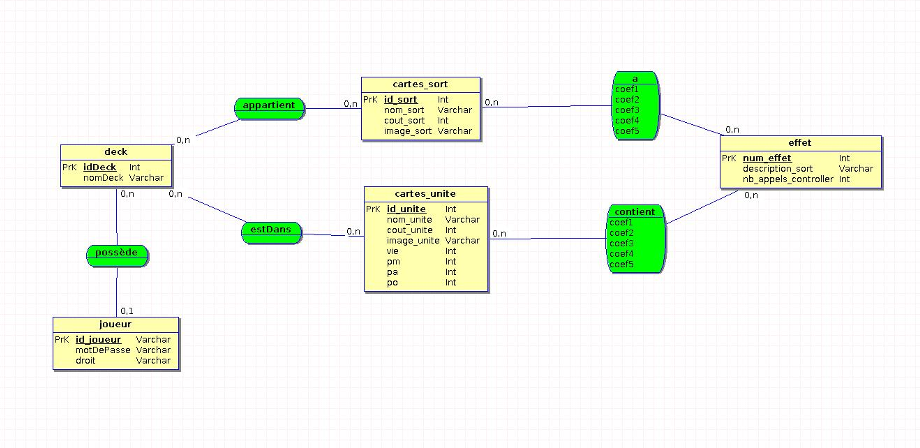
\includegraphics[scale=0.4]{Assets/MCD.png}
        \caption{MCD du jeu \textit{data wars}}
        \label{fig1}
      \end{center}
    \end{figure}
    
    \begin{itemize}
      \item Joueur et Deck
      \item Cartes
      \item Effets
    \end{itemize}

    \section{Joueur et deck}
      La base de données va stocker le nom des joueurs et leurs mots de passe ainsi que les droits pour les accès au site web. Un deck sera relié à chaque joueur.
    
    \begin{figure}[th]
      \begin{center}
        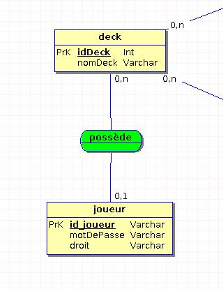
\includegraphics[scale=0.6]{Assets/MCD_Joueur.png}
        \caption{Zoom sur le joueur et le deck}
        \label{fig2}
      \end{center}
    \end{figure}
    
    
    \section{Les cartes}
      Il existe deux types de cartes, les cartes sorts et les cartes unités. Les cartes sorts contiennent moins d'informations que leurs homologues. Elles ne contiennent que le coût, le chemin vers l'image et le nom en plus de leurs identifiants. Les cartes unités, elles, contiennent les caractéristiques nécessaires à la création des unités. Elles sont liées au deck, chacune via une association. Puis d'un autre coté, elles sont aussi reliées aux effets.
      
    \begin{figure}[th]
      \begin{center}
        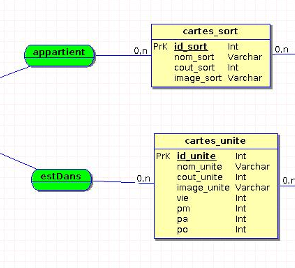
\includegraphics[scale=0.6]{Assets/MCD_Cartes.png}
        \caption{Zoom sur les cartes}
        \label{fig3}
      \end{center}
    \end{figure}
      
      \section{Les effets}
        Les effets sont les derniers éléments de cette base de données. Chaque élément \textit{<<effet>>} inséré dans la base de données correspond à un type d'effet, par exemple : <<soigne de X points de vies>> ou <<inflige X points de dégâts>>. C'est lorsque ce type \textit{<<effet>>} sera lié à une carte via les associations \textit{<<a>>} et \textit{<<contient>>} que les valeurs remplaceront les <<X>> via les coefficients. Les coefficients utilisés (c'est-à-dire dans nos deux exemples, seulement le premier coefficient) devront être remplis et les autres seront mis à -1. La variable \textit{nb\_appels\_controller} sert elle, à indiquer le nombre de clics nécessaires pour jouer une carte qui contient cet effet.

    \begin{figure}[th]
      \begin{center}
        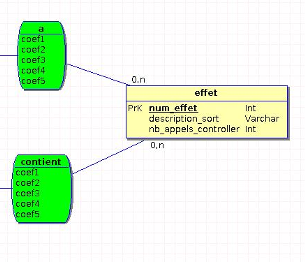
\includegraphics[scale=0.6]{Assets/MCD_Effet.png}
        \caption{Zoom sur les effets}
        \label{fig4}
      \end{center}
    \end{figure}

\chapter{Le modèle}
    Le modèle est composé d'un ensemble de classes toutes reliées de près, ou de loin, à la classe dite <<mère>> du modèle la classe \textit{Game}. Nous pouvons ensuite décomposer le schéma UML (\textit{Figure ~\ref{fig5}}) en trois gros blocs :
    \begin{itemize}
      \item Le bloc concernant la grille (la carte)
      \item Le bloc concernant les joueurs
      \item Le bloc concernant le serveur 
    \end{itemize}
    Le troisième bloc sera détaillé en aval. Nous allons ici nous concentrer sur la partie jeu du programme, soit les deux premières parties.
    
    \begin{figure}[th]
      \begin{center}
        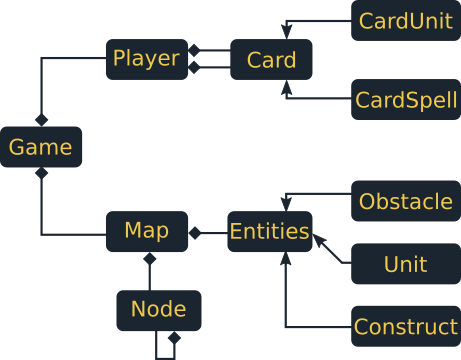
\includegraphics[scale=0.4]{Assets/UML.png}
        \caption{Le schémas UML du jeu}
        \label{fig5}
      \end{center}
    \end{figure}
    
    \section{Le bloc grille}
        La carte du jeu, que nous appellerons ici <<grille>> ou encore \textit{<<map>>} et l'élement essentiel du bloc grille. Cette objet Java contient un tableau à deux dimensions qui représente la grille ainsi que d'autre attributs qui seront expliqués plus en détails par la suite. Cette classe contient la plupart des fonctions de traitement des entités, qui sont les éléments qui composent la grille. Rentrons plus en détails dans ce bloc.
    \begin{figure}[th]
      \begin{center}
        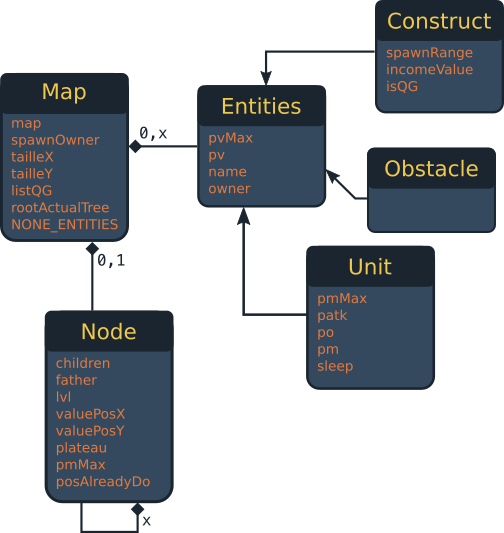
\includegraphics[scale=0.4]{Assets/umlBlocGrille.png}
        \caption{Zoom sur le bloc grille}
        \label{fig6}
      \end{center}
    \end{figure}
        \subsection{Les entités}
          \begin{center}
           \textit{Classe : Entities, Unit, Construct, Obstacle}
          \end{center}
          Les entités sont les éléments contenus par la grille. Elle sont de type \textit{entities}, c'est-à-dire qu'elles appartiennent à cette classe. Cette classe contient les propriétés suivantes :
          \begin{itemize}
            \item <<points de vie actuels>>
            \item <<points de vie>>
            \item <<nom>>
            \item <<propriétaire>>
          \end{itemize}
          Il faut savoir que toutes les propriétés <<points de vie>> sont dédoublées. En effet, il faut garder pour la propriété <<points de vie>> la valeur de départ pour ne pas dépasser cette limite si nous soignons l'unité.
          La classe \textit{Entities} va avoir trois subdivisions, que l'on appele <<type d'entité>> :
          \begin{description}
            \item[Les unités :] modélisées par la classe \textit{Unit}, elle correspond aux unités que le joueur peut poser. Elles ont des attributs supplémentaires, les <<points de mouvement>> et <<points de mouvement maximum>>, ainsi que des points d'attaque. Elles peuvent attaquer les autres unités qui perdront des points de vie et pourront potentiellement contre-attaquer.
            \item[Les obstacles :] modélisés par la classe \textit{Obstacle}, correspond aux obstacles qui sont là pour bloquer les unités.
            \item[Les bâtiments :] modélisés par la classe \textit{Construct}, elle correspond aux QG et aux bâtiments de ressources. Ils ont plusieurs attributs supplémentaires tels que le \textit{spawnrange} qui détermine la zone où nous pouvons placer des unités quand le bâtiment nous appartient, l'\textit{incomeValue} qui est le nombre de ressources données par ce bâtiment par tour. Enfin la variable \textit{isQg} détermine si ce bâtiment est un QG ou non.
          \end{description}
        \subsection{L'accès aux unités}
          \begin{center}
           \textit{Classe : Map}
          \end{center}
          Pour accéder aux unités, il faut passer par l'attribut \textit{map} de la classe \textit{Map}. Pour ce repèrer, il faut comprendre le système algorithmique de gestion des coordonnées (\textit{Figure~\ref{xyExample}}). Or, lors de l'appel à certaines méthodes, l'utilisateur doit envoyer un tableau de coordonnées sous la forme [x,y]. Il faut donc faire attention à ne pas mélanger les deux.
        
        \begin{figure}[th]
          \begin{center}
            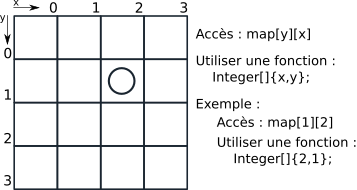
\includegraphics[scale=0.6]{Assets/xyExemple.png}
            \caption{Exemple d'accès aux unités}
            \label{xyExample}
          \end{center}
        \end{figure}
        
        
        \subsection{Les déplacements}
        \begin{center}
          \textit{Classe : Map - Fonction : setUnitTreeOfMove(), move()}
        \end{center}
          La gestion du plus court chemin et des obstacles a nécessité la création d'un système d'arbre afin de calculer les différentes possibilités de déplacements et de choisir le chemin le plus optimisé. Pour créer cet arbre, nous avons créé une classe \textit{Node} qui va gérer ce traitement. En fonction d'une coordonnée passée en paramètre, ainsi que d'un nombre de points de mouvement, elle peut calculer l'arbre des possibilités (\textit{Figure~\ref{treeExample}}), où chaque nœud correspond à une position. De plus, elle va nous générer une liste contenant toutes les positions accessibles par l'unité afin de pouvoir l'afficher. Ensuite cet arbre subira un parcours en largeur afin de déterminer le plus court chemin (\textit{Figure~\ref{parcourExample}}) pour aller à une position, en récupèrent de nombre de points de mouvements nécessaire. Le déplacement permet également, si l'unité attaque au corps à corps et si la position de destination est occupée par une autre entité, de l'attaquer.
          
          \begin{figure}[th]
          \begin{center}
            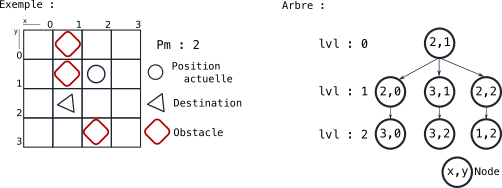
\includegraphics[scale=0.6]{Assets/treeExample.png}
            \caption{Exemple d'une création d'arbre via la classe \textit{Node}}
            \label{treeExample}
          \end{center}
        \end{figure}
            
        \begin{figure}[th]
          \begin{center}
            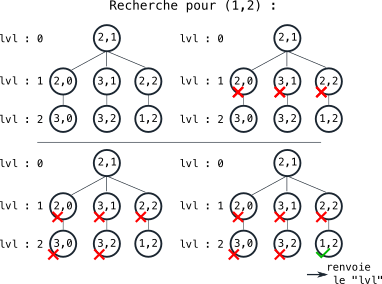
\includegraphics[scale=0.6]{Assets/parcourTree.png}
            \caption{Exemple d'un traitement de l'arbre}
            \label{parcourExample}
          \end{center}
        \end{figure}
        

      
        \subsection{Utilisation des nodes}
        \begin{center}
          \textit{Classe : Node - Fonction : calcNextLevel(), searchLowCostPath(), searcheLowCostPathForAttack(), setUpTreeOfMovement()}
        \end{center}
          L'utilisation de la classe \textit{Node} nécessite une certaine rigueur de part sa construction. En effet, pour fonctionner celle-ci à besoins de plusieurs variables dites \textit{<<static>>} que tout les nœuds se partagent de façon à traiter l'arbre. Il faut donc respecter une procédure stricte afin d'initialiser le premier nœud. Il faut donc appeler la méthode \textit{<<static>> setUpTreeOfMovement()} de la classe \textit{Node} qui retourne le nœud <<racine>> de l'arbre résultant des paramètres données. C'est depuis ce nœud que vous pourrez appeler les différents services de la classe.
        
        \subsection{L'attaque}
        \begin{center}
        \textit{Classe : Map - Fonction : attack()}
        \end{center}
        L'algorithme détermine si la carte est une unité de corps à corps, ou de distance. Puis vérifie si celle-ci a la portée pour attaquer, avant d'infliger les dégats si nécessaire et de regarder si l'unité adverse doit contre-attaquer ou non.
          
        \subsection{L'apparition d'unités}
          \begin{center}
          \textit{Classe : Map - Fonction : spawn()}
          \end{center}
            Lorsqu'une carte est jouée et que, par la même occasion, une unité est créée nous devons vérifier si le joueur peut placer l'unité à l'endroit qu'il souhaite. Pour ce faire il va d'abord regarder si la case n'est pas déjà occupée. Si ce n'est pas le cas, alors nous allons regarder si le joueur a l'autorisation de poser une unité sur cette case. C'est l'attribut \textit{spawnOwner}, qui est un tableau à deux dimensions contenant le même nombre de cases que la grille, et qui dit sur chaque case, qui en est le détenteur. Si le joueur possède cette case, alors il peut poser une unité dessus.

        
        \subsection{La capture}
          \begin{center}
           \textit{Classe : Map - Fonction : tryCaptureConstruct()}
          \end{center}
          Lorsqu'une unité se déplace à côté d'un bâtiment, elle peut le capturer. Si les conditions sont réunies, alors ce bâtiment est capturé et les cases de la variable \textit{spawnOwner} adjacentes à <<n>> distance de ce bâtiment sont converties au joueur. Les <<n>> de distance sont égales à la variable \textit{spawnRange} du bâtiment. De plus, le joueur devient le propriétaire du bâtiment (via \textit{setOwner()}).
      
      \section{Le bloc joueur}

        \subsection{Les cartes}
          \begin{center}
           \textit{Classe : Card, CardSpell, CardUnit}
          \end{center}
          Les cartes sont les objets correspondant aux cartes vues dans la base de données plus haut. Il en existe deux types :
          \begin{description}
            \item[Carte unité :] ces cartes ont la particularité de contenir, en plus des caractéristiques des cartes, toutes les caractéristiques nécessaires à la création d'une nouvelle unité. Elles nécessitent un clic supplémentaire sur la grille, par rapport aux clics nécessaires pour lancer son effet (\textit{nb\_appels\_controller}), pour être jouées (pour dire où doit être posée cette unité).
            \item[Carte sort :]  ce sont les cartes qui ne vont pas créer d'unités, elles n'ont pas de caractéristiques supplémentaires, mais doivent pouvoir être différenciées de l'autre type afin de choisir quelle image de carte doit être affichée.
          \end{description}
         
         \begin{figure}[th]
          \begin{center}
            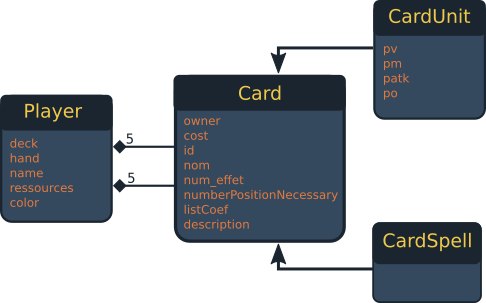
\includegraphics[scale=0.4]{Assets/umlBlocCarte.png}
            \caption{Zoom sur le bloc joueur}
            \label{fig7}
          \end{center}
        \end{figure}
             
          \subsection{Les joueurs}
            \begin{center}
            \textit{Classe : Player}
            \end{center}
            Les joueurs ont une <<main>> qui contient cinq cartes (attribut \textit{hand}), et un <<deck>> qui en contient cinq également (attribut \textit{deck}). Les joueurs possèdent également un nom,  une couleur (en chaine de caractères) et un nombre de ressources. C'est de cette classe que vont être jouées les cartes.
            
          \subsection{Jouer une carte}
            \begin{center}
            \textit{Classe : Player, Card - Fonction : doEffect() , playCard(),  spawn()}
            \end{center}
            La notion de jouer une carte va faire appelle à plusieurs engrenages du système.Tout d'abord la fonction \textit{playCard()} va récupérer une liste de coordonées construite par le controlleur en fonction de l'attribut \textit{nomberPositionNecessary} de la carte. Tout d'abord le programme va regarder si la carte peut-être jouée, c'est-à-dire si le joueur à le nombre de ressources nécessaire pour jouer la carte. Ensuite, l'algorithme va déterminer si la carte est une carte unité ou une carte sort. Si la carte est une unité, cette carte va créer l'unité en récupérant et enlevant la première position de la liste de position. Puis le traitement ce rejoint entre les deux types de carte en appelant la fonction \textit{doEffect()}.
            
          \subsection{Jouer un effet}
            \begin{center}
            \textit{Classe : Card - Fonction : doEffect()}
            \end{center}
            Jouer un effet est la partie qui lie le plus la base de données au jeu, et par conséquence, demande une grande rigueur dans l'insertion des effets et des cartes dans celle-ci. En effet, lors de l'appel à la méthode \textit{doEffect()}, celle-ci va regarder via l'attribut \textit{num\_effet} le numéros de l'effet, qui correspond à l'identifiant de celui-ci dans la base de données. En fonction de ce chiffre, la méthode va faire le traitement adapté à cette identifiant.

         \begin{figure}[th]
          \begin{center}
            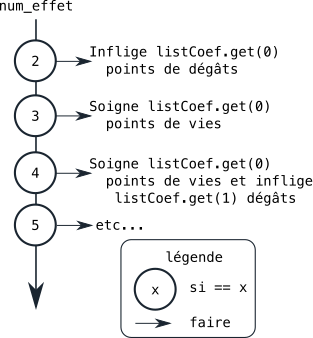
\includegraphics[scale=0.5]{Assets/decisionEffet.png}
            \caption{Schémas du traitement de la fonction \textit{doEffect()}}
            \label{decisionEffet}
          \end{center}
        \end{figure}
      
          \subsection{Mélanger les cartes}
            \begin{center}
            \textit{Classe : Player - Fonction : shuffle()}
            \end{center}
              La méthode \textit{shuffle()} va remettre toute les cartes dans le <<deck>> avant de les mélanger et de reprendre cinq cartes dans la <<main>>.
            
    \section{Le jeu}
     Nous allons maintenant parler de la classe \textit{Game}.
      
     \begin{figure}[th]
        \begin{center}
          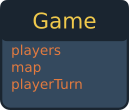
\includegraphics[scale=0.4]{Assets/UMLGame.png}
          \caption{Zoom sur la classe \textit{Game}}
          \label{figUMLGame}
        \end{center}
      \end{figure}
      
      \subsection{Savoir qui joue}
        \begin{center}
        \textit{Classe : Game - Fonction : getPlayerTurn()}
        \end{center}
        La classe \textit{Game} contient une liste de joueur ainsi qu'une variable appelée \textit{playerTurn}. Cette variable est utilisée comme un curseur qui indique quel élément de la liste doit jouer.

      \subsection{Récupération des cartes}
        \begin{center}
        \textit{Classe : Game - Fonction : setDeckPlayerByName()}
        \end{center}
        C'est le serveur qui est chargé de la récupération des cartes depuis la base de données. Il va ensuite les envoyer au jeu grâce à la méthode \textit{setDeckPlayerByName()}. Cette méthode prend le nom d'un joueur ainsi qu'un tableau de cartes en paramètre, et va donc ajouter celles-ci au joueur du modèle ayant ce nom. Si aucun joueur ne correspond, la fonction nous informe via un booléen de l'échec de la méthode.
        
        \subsection{Initialisation de la carte}
        \begin{center}
        \textit{Classe : Game - Fonction : initMap()}
        \end{center}
        La création de la carte ne dépend que d'un seul élément, le nombre de joueur. Selon celui-ci, la carte sera créés suivant un modèle codé dans le programme.
        
        \subsection{La gestion de la fin du tour}
        \begin{center}
        \textit{Classe : Game - Fonction : endTurn()}
        \end{center}
        La fonction \textit{endTurn()} est appelée à chaque fin de tour de façon à débloquer les unités du joueur (booléen \textit{sleep}), à remettre leurs points de mouvements à leurs maximums et de changer de joueur en incrémentant la variable \textit{playerTurn}. 
        
      \section{Les exceptions}
        Nous allons ici détailler les différentes exceptions propre au modèle.
        \begin{description}
          \item[EffectException : ]Déclenché lorsqu’un effet n’est pas utilisé dans de bonne condition, (exemple : les coordonnées sélectionnées ne contiennent pas d’unités).
          \item[MoveException : ]Déclenché lorsqu'une unité essaie de ce déplacer sur une case déjà occupé, ou qu'il ne peut pas atteindre.
          \item[PlayCardException : ]Déclenché si un joueur tente de jouer une carte qui coûte plus que le nombre de ressources dont il dispose.
          \item[RangeException : ]Déclenché par une unité qui tente d'attaquer une autre, qui n'est pas à sa portée.
          \item[SpawnExcpetion :]Déclenché par un joueur qui tente de poser une unité sur une case qui est déjà occupée ou qui n'appartient pas à celui-ci.
        \end{description}
        




\chapter{Partie réseau}

\section{Modélisation des classes de réseau}
Dans cette partie les classes principales du client et du serveur seront présenté, ainsi que l'organisation entre elles.
\subsection{UML de gestion des clients pour le serveur}

    \begin{figure}[th]
      \begin{center}
        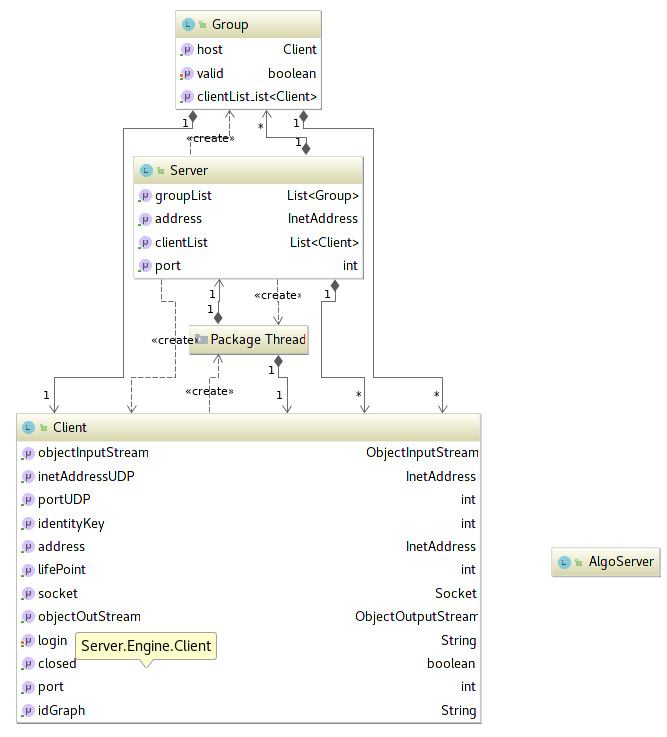
\includegraphics[scale=0.3]{Assets/UML_serveur.png}
        \caption{UML du serveur}
        \label{UML du serveur}
      \end{center}
    \end{figure}
    
    
    Comme illustré sur le diagramme ULM (\textit{figure~\ref{UML du serveur}}) le serveur contient des clients et des groupes. Les groupes contiennent eux même des clients. Un groupe possède en variable d’instance son hôte. Un client possède les flux objets, son socket et ses coordonnées pour le transport UDP. Le serveur lui possède son socket serveur TCP et UDP.


\subsection{UML de gestion des données pour les clients}
 \begin{figure}[th]
      \begin{center}
        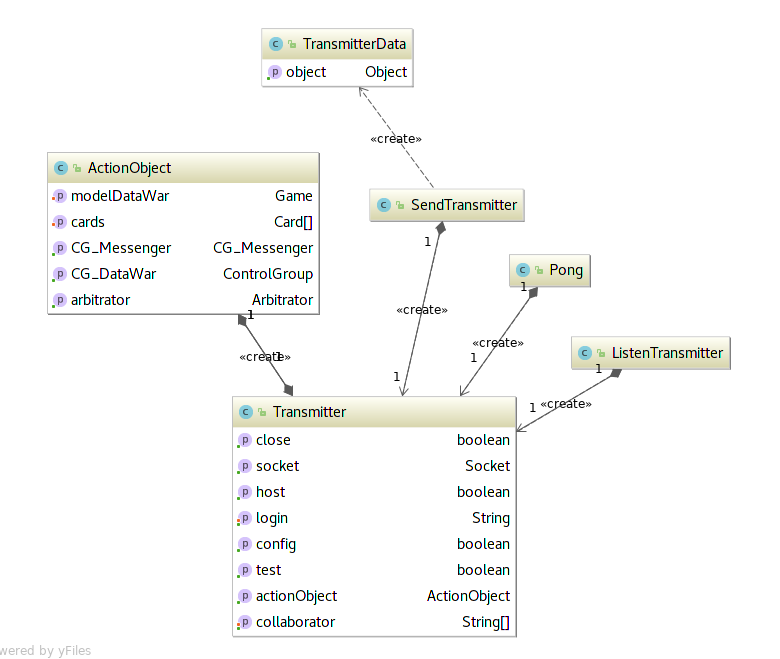
\includegraphics[scale=0.3]{Assets/UML_client.png}
        \caption{UML du client}
        \label{UML du client}
      \end{center}
    \end{figure}
    
  Comme illustré sur le diagramme ULM (\textit{figure~\ref{UML du client}}) le \textit{Transmitter} a pour variable d’instance son socket de connexion, ses flux objets, la liste des logins des membres du groupe. La variable host permet de savoir le mode hôte ou invité sur le groupe et la variable test sert aux tests logiciels. Un \textit{Transmitter} possède un \textit{ActionObject} et un \textit{ActionObject} possède un \textit{Transmitter}. La classe \textit{ActionObject} contient les contrôles groupes des applications qu’elle fait fonctionner en réseau : \textit{Messenger}, et le \textit{DataWar}.



\section{Les classes annexes}

Cette partie présente les classes "accessoire" du serveur.

\subsection{Visualisation de la situation du serveur}

    \begin{figure}[th]
      \begin{center}
        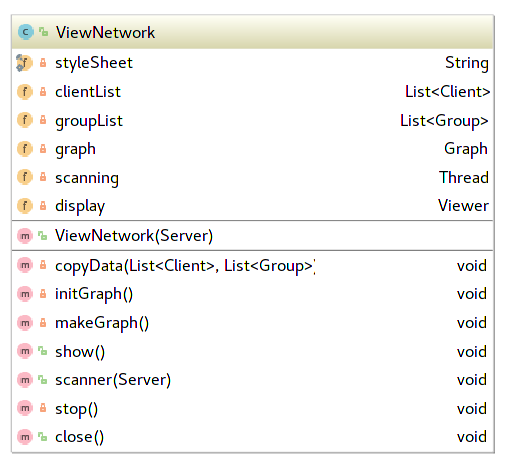
\includegraphics[scale=0.3]{Assets/UML_Network.png}
        \caption{Classe ViewNetwork}
        \label{Classe ViewNetwork}
      \end{center}
    \end{figure}
    
    La classe \textit{ViewNetwork} (voir la \textit{figure~\ref{Classe ViewNetwork}}) permet une visualisation en temps réel de la situation du serveur. Elle montre dans une fenêtre un graphe avec pour nœud les clients et leur groupe pour liaisons. Le graphe est créé avec la librairie \textit{GraphSteam}. Lors de la création de la classe un thread est lancé pour réactualiser le graphe sur l’état du serveur. La fréquence de réactualisation est de 500 millisecondes.

\subsection{Communication avec la base de donnée}

  \begin{figure}[th]
      \begin{center}
        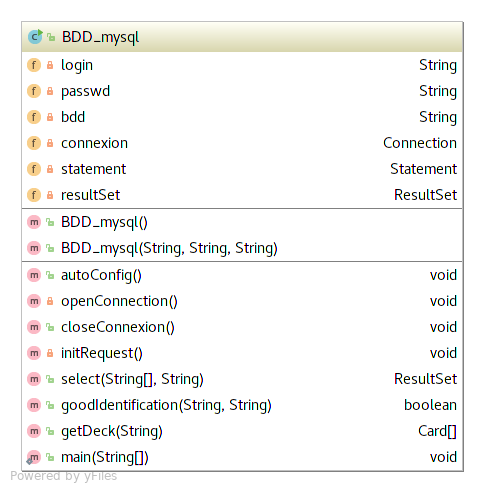
\includegraphics[scale=0.3]{Assets/UML_BDD.png}
        \caption{Classe BDD\_mysql}
        \label{Classe BDD_mysql}
      \end{center}
    \end{figure}
    
    La classe \textit{BDD\_mysql} (voir la \textit{figure~\ref{Classe BDD_mysql}}) permet d’accéder simplement à la base de donnée du serveur. La classe utilise le package \textit{mysql\_connector} pour accéder à la base de donnée et exécuter les recettes SQL. La classe possède des fonctions permettant de savoir si un utilisateur est correctement identifié, ou encore la récupération du deck d’un joueur sous forme objet.




\section{Organisation et fonctionnement des communications}

\subsection{Organisation des communications}
Dans cette partie sera présenté le fonctionnement et l’organisation des communications du module de gestion du réseau.

\subsubsection{Organisation physique des communications}

L’organisation physique des communications est représenté sur le schéma en \textit{figure~\ref{schémaCom}} avec sa légende en \textit{figure~\ref{leSchémaCom}}
  
  \begin{figure}[th]
      \begin{center}
        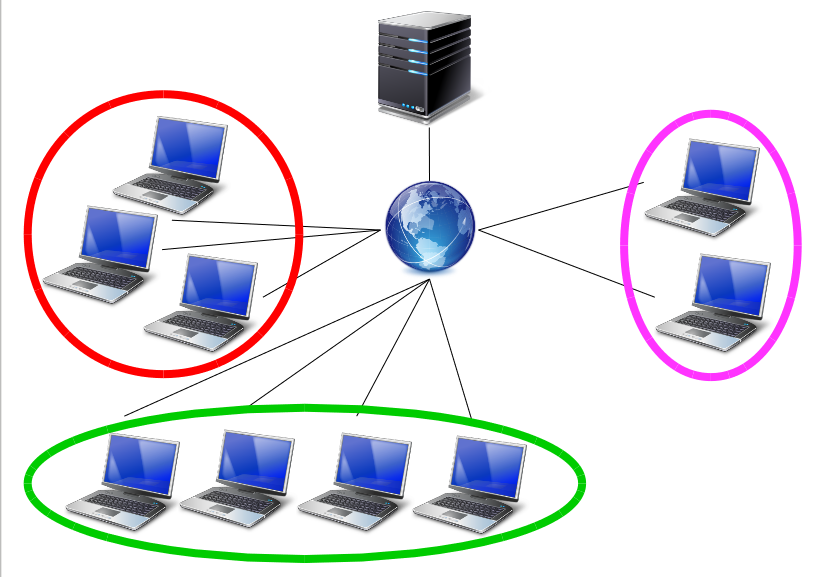
\includegraphics[scale=0.3]{Assets/s_r_1.png}
        \caption{Schéma montrant les communications physique}
        \label{schémaCom}
      \end{center}
    \end{figure}

   \begin{figure}[th]
      \begin{center}
        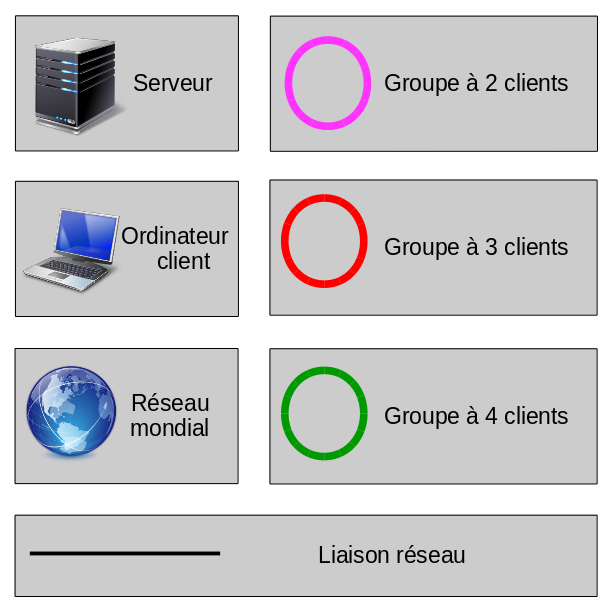
\includegraphics[scale=0.2]{Assets/l_r_1.png}
        \caption{Légende du schéma montrant les communications physique}
        \label{leSchémaCom}
      \end{center}
    \end{figure}
    
  
  Une fois que les groupes sont configurés et créé, le serveur établit les communications entre les différents membres d’un groupe. Le serveur a donc un rôle de relai.
Ce fonctionnement par relai permet de communiquer dans des zones avec des par-feus très restrictifs.
Le serveur est capable de gérer plusieurs groupes en même temps et de différente taille entre 2 et 4 membres. Deux clients appartenant chacun à un groupe différant ne peuvent pas communiquer entre eux.

\subsubsection{Organisation logicielle des communications}

  Un client communique simultanément avec tous les autres clients, ils ne peuvent pas parler un à un. 
Ceci pour faciliter simplement la synchronisation des données du modèle du jeu, et la gestion des avaries lors de déconnexion éventuel. De cette façon le client n’a pas besoin de savoir qui est encore connecté pour envoyer les données. (la synchronisation et les avarie seront expliqué plus tard).
  
\subsection{Fonctionnement des communications}

\subsubsection{Classes de communication}
Le tableau \ref{tab1comClasses} récapitule les classes pour transmettre des objets.

  \begin{table}
    \begin{center}
      \begin{tabular}{|c|c|c|}
         \hline \textbf{Action}&\textbf{Classe du serveur}&\textbf{Classe du client} \\
         \hline Attendre de recevoir&\textit{ListenClient\_Wait}&- \\
         \hline Attendre d’envoyer&\textit{SendClient\_Wait}&- \\
         \hline Recevoir&\textit{ListenClient}&\textit{ListenTransmitter} \\
         \hline Envoyer&\textit{SendClient}&\textit{SendTransmitter}\\
         \hline
      \end{tabular}
      \caption{Tableau récapitulant les classes pour les transmissions objet}  
      \label{tab1comClasses}
    \end{center}
  \end{table}
  
  Les classes pour attendre de recevoir ou d’envoyer des données sont les classes mères des classes pour envoyer ou recevoir des données. La différence avec les classes filles est qu’elles implémentes \textit{Runnable} pour pouvoir être threader.

\subsubsection{Procédure de communication communication entre membre d’un groupe}
Cette procédure permet à un client de communiquer avec les autres membres de son groupe.
\begin{description}
  \item[1) Envoie des données du client vers le serveur]
    \textit{\\Classe : Transmitter - Fonction : speakTransmitters()\\}
	  Pour envoyer un objet quelconque il suffit d’appeler cette méthode et de passer en paramètre l’objet à envoyer à destination du serveur pour une retransmission. Cette méthode est \textit{synchronized} pour être certain que l’on ne puisse pas envoyer des données dans le désordre ou avoir des conflits avec d’autre méthode de communication. Les données à envoyer sont encapsulés dans une classe \textit{TransmitterData}.
	
	\item[2) Réception des données des clients]
	\textit{\\Classe : ListenClient - Fonction : run()\\}
	  Le serveur attend des objets sur le flux objet de chaque client avec un thread d'écoute pour chacun.
Dans cette méthode lorsqu’un objet est reçu, le serveur vérifie le type de donnée avant de la retransmettre. Si un nombre trop important d’erreur venait à se produire, la méthode fermerait le socket du client en question.

  \item[3) Retransmission des données du serveur vers les clients]
  \textit{\\Classe : Group - Fonction : clientSpeakGroup()\\}
    Une fois la réception d’un objet  \textit{TransmitterData} le serveur retransmet les données aux autres membres du groupe. Cette méthode est elle aussi  \textit{synchronized} pour les mêmes raisons que la méthode précédente. Pour réaliser son traitement la méthode à besoin de l’objet à transmettre et du client émetteur pour ne pas lui retourner les données.
    
  \item[4) Réception des données du serveur]
  \textit{\\Classe : ListenTransmitter - Fonction : run()\\}
    Le client attend des objets dans cette fonction. Si un objets est reçu il est envoyé dans la classe \textit{Transmitter} par la méthode \textit{readObject()} pour être traité. Si des erreurs sont constatés le socket est fermé.
\end{description}

\subsubsection{Procédure de communication direct avec le serveur}
  Cette procédure permet à un client de réaliser des actions enregistrées dans le serveur par le développeur.

\begin{description}
  \item[1) Envoi du signal au serveur]
    \textit{\\Classe : Transmitter - Fonction : speakTransmitters()\\}
	  Cette méthode à pour bute de transmettre au serveur le signal (un \textit{Integer}) au serveur. Pour cela la méthode encapsule le signal dans l’objet \textit{ServerMessage}. L’objet est transmit par les flux objets du \textit{Transmitter} dans un thread.
	
	\item[2) Réception du signal par le serveur]
	\textit{\\Classe : ListenClient - Fonction : run()\\}
	  La réception du signal ce fait ici au même endroit que la réception des données de groupe. Si l’objet reçu est une instance de  \textit{ServerMessage}, alors il est transmit à la classe serveur pour être traité.

  \item[3) Traitement du signal]
  \textit{\\Classe : processingMessage - Fonction : run()\\}
  Cette méthode exécute l’instruction correspondante au numéro de signal dans l’objet \textit{ServerMessage}.
\\Pour le moment deux signaux sont répertoriés dans le tableau \ref{tab2signal}.

\newcolumntype{M}[1]{>{\raggedright}m{#1}}
\begin{table}
    \begin{center}
      \begin{tabular}{|l|M{12cm}|}
         \hline \textbf{Signal}&\textbf{Action}\tabularnewline
         \hline 6&Ordonne la fermeture du signal si le code contenue dans la classe est correcte.\tabularnewline
         \hline 5&Recherche les cartes du groupe dans la base de donnée avec la classe \textit{BDD\_mysql} et la méthode \textit{getDeck()}. Puis les cartes sont retournées par les flux objet à l’émetteur du signal.\tabularnewline
         \hline
      \end{tabular}
      \caption{Tableau récapitulant les type de signaux du serveur}  
      \label{tab2signal}
    \end{center}
  \end{table}
\end{description}

  
\subsection{Protocole de création d’un groupe}

  Sur l'organigramme en figure \ref{organiGroupe} est présenté la procédure de création d’un groupe de jeu sur le serveur et sa légende sur le tableau \ref{tabOrganigramme}.

  \begin{figure}[th]
      \begin{center}
        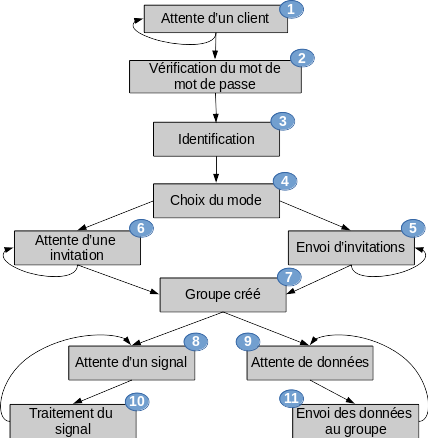
\includegraphics[scale=0.9]{Assets/creationGroup.png}
        \caption{Organigramme montrant les étapes de la création d'un groupe}
        \label{organiGroupe}
      \end{center}
    \end{figure}

\newcolumntype{M}[1]{>{\raggedright}m{#1}}
  
  \begin{table}
    \begin{center}
      \begin{tabular}{|l|M{9cm}|M{2.7cm}|}
      
       \hline \textbf{N}&\textbf{Action}&\textbf{Classes utilisées}\tabularnewline
         
        \hline 
        1&Cette étape consiste à attendre un client, créer un socket, puis ouvrir un flux objet provisoire entrant. Si le port et l’adresse sont enregistrés dans la liste forcing alors le client est déconnecté.&\textit{WaitClients}\\\textit{Server}
        \tabularnewline

        
        \hline 
        2&Le serveur attend la clef d’accès envoyer par le client.
Si la clef est incorrecte le client est déconnecté, puis son adresse et son port sont stockés dans la liste forcing pour que la personne ne puisse pas forcer la clef. Sinon les flux objet entrant et sortant sont créés ainsi que les classes \textit{Ping} et \textit{Pong}.&\textit{Server}\\\textit{Ping}/\textit{Pong}\\\textit{Client}\\\textit{BDD\_mysql}
        \tabularnewline
        
        \hline
        3&L’étape d’identification consiste à recevoir le login et le mot de passe du client.\\
        -Si elle ne correspond pas à la base de donnée ou si la même personne est déjà connecté le socket est fermé.\\
        -Si l’identification est correcte un message de sucés est envoyé.&\textit{Server}\\\textit{Client}\\\textit{InfoProtocol}
        \tabularnewline
        
        \hline
        4&Cette étape consiste à demander au client quelle mode de création de groupe souhaite-t-il.\\
Si le client revoit yes, alors un groupe est créé ou il en est hôte. Sinon le client est mis en attente d’acceptation d’un groupe.&\textit{Server}\\\textit{Group}\\\textit{InfoProtocol}
        \tabularnewline
        
        
        \hline
        5&Une liste de tout les clients en attente d’invitation est envoyé a l’hôte. L’hôte peut envoyer une invitation à un client en attente d’invitation en envoyant le nom de la personne concerné au serveur, puis le serveur transmet l’invitation. L’hôte peut envoyer le message de fin de configuration et si la taille du groupe est entre 2 et 4 personnes le groupe est validé.&\textit{Server}\\\textit{Client}\\\textit{InfoProtocol}
        \tabularnewline
        
        \hline
        6&Le serveur transmet toutes les invitations au client avec un délai de 12 secondes maximum pour répondre.
Si le client renvoi l’invitation il est placé dans le groupe de l’émetteur et attend la validation du groupe.
Si il la refuse il ne renvoie rien.
Si le temps est dépassé le serveur n’acceptera pas une éventuelle acceptation cette invitation.&\textit{Server}\\\textit{Group}\\\textit{Client}\\\textit{Transmitter}\\\textit{InfoProtocol}
      
        \tabularnewline
        
        \hline
        7&Lorsque l’hôte valide le groupe, un message de confirmation de sa création est envoyé à tous ses membres. Ainsi qu’une liste de nom de tout ses membres.&\textit{Server}\\\textit{Group}\\\textit{InfoProtocol}
        \tabularnewline
        
        \hline
        8&Le serveur attend un signal contenu dans l’objet \textit{ServerMessage} émis par un des membres du groupe.&\textit{ServerMessage}\\\textit{Server}
        \tabularnewline
        
        \hline
        9&Le serveur attend des donnés contenus dans l’objet \textit{TransmitterData}.&\textit{TransmitterData} \\\textit{Server}
        \tabularnewline
        
        \hline
        10&Suivant ce signal le serveur exécute une procédure bien précise.&\textit{Server}\\\textit{Client}
        \tabularnewline
        
        \hline
        11&Le serveur retransmet les données aux membres du groupe.&\textit{Group}
        \tabularnewline
        
        \hline
      
      \end{tabular}
      \caption{Tableau expliquant les étapes de l'organigramme \textit{(figure~\ref{organiGroupe})}}  
      \label{tabOrganigramme}
    \end{center}
  \end{table}


\section{Principe et fonctionnement de la synchronisation par le réseau}

  Le principe de la synchronisation par réseau est simple. Le but est de synchroniser les modelés de chaque joueur. De cette manière le module de réseau est indépendant du jeu. La synchronisation fonctionne parfaitement pour tous les jeux tour par tour. Ce principe de fonctionnement est très simple, mais son défaut est que le modèle du jeu doit être léger et \textit{serializable}.
\\
Le schéma en figure \ref{syncros} avec sa légende \textit{(Figure~\ref{syncroslegende})} et ses étape \textit{(Tableau~\ref{syncros})} illustre son fonctionnement.
  \begin{figure}[th]
      \begin{center}
        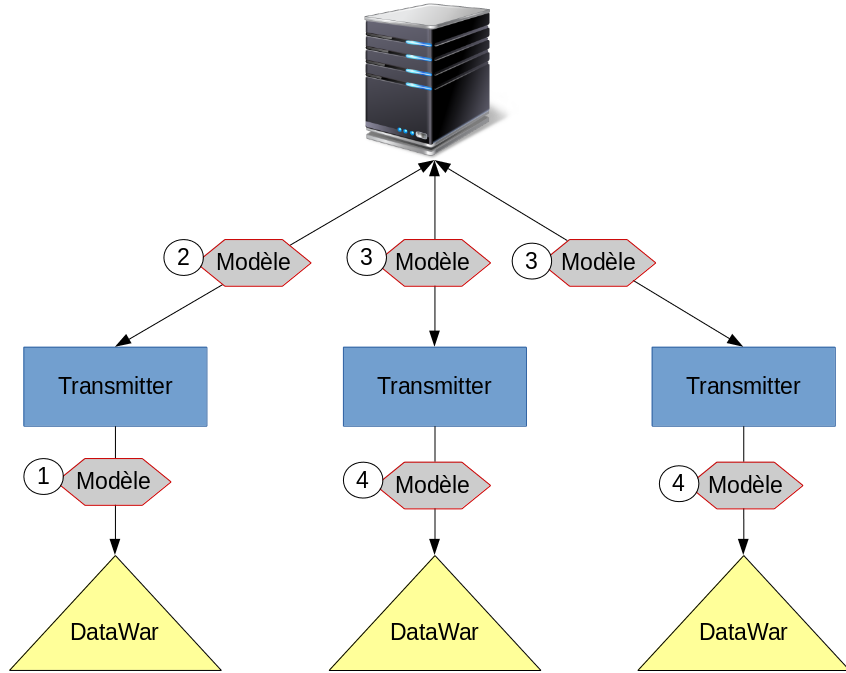
\includegraphics[scale=0.4]{Assets/s_r_2.png}
        \caption{Schéma illustrant la synchronisation par le réseau}
        \label{syncros}
      \end{center}
  \end{figure}
  
  \begin{figure}[th]
      \begin{center}
        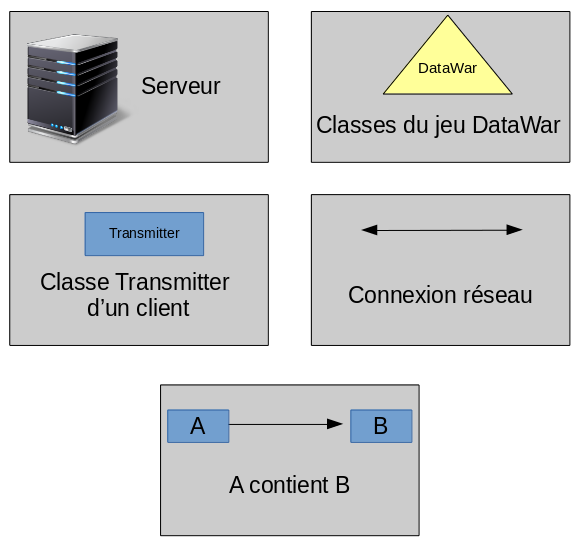
\includegraphics[scale=0.3]{Assets/l_r_2.png}
        \caption{Légende du schéma \ref{syncros}}
        \label{syncroslegende}
      \end{center}
  \end{figure}
  
  \newcolumntype{M}[1]{>{\raggedright}m{#1}}
    \begin{table}
      \begin{center}
        \begin{tabular}{|l|M{12cm}|}
           \hline \textbf{Étape}&\textbf{Action}\tabularnewline
           
           \hline 
           1&Le joueur vient de terminer son tour. L’envoi de son modèle de jeu est donc ordonnée par un contrôleur du \textit{DataWar}. Le modèle est transmit au \textit{Transmitter}.
           \tabularnewline
           
           \hline 
           2&Le \textit{Transmitter} se charge de \textit{serializer} le modèle du \textit{DataWar}. Puis il le transmet au serveur.
           \tabularnewline
           
           \hline
           3&Le serveur retransmet le modèle aux membres du groupe.
           \tabularnewline
           
           \hline
           4&Le \textit{Transmitter} provoque la mise à jour du modèle par rapport au modèle reçu.
           \tabularnewline
           
           \hline
        \end{tabular}
        \caption{Étape de la figure \ref{syncros}}  
        \label{tab3Etape}
      \end{center}
    \end{table}


\section{La gestion des erreurs et avaries}
  Il va de soi que si un client est déconnecté subitement, si il provoque des anomalies, ou voir même si il souhaite détourné le programme, le serveur ne doit pas arrêter de fonctionner. Dans cette partie sera présenté les différents mécanismes de réparation.

\subsection{Gestion des déconnexions}
  Lorsqu’un client est identifié par le serveur comme déconnecté il doit être détruit, ses threads doivent être terminé et les contraintes avec un groupe éventuel doivent être géré.

\subsubsection{Suppression des clients et groupes du serveur}

\begin{description}
  \item[La suppression des clients]
  \textit{\\Classe : Serveur – Fonction : deleteClient()\\}
    Cette méthode a pour but de supprimer du serveur le client passé en paramètre. Pour cela la méthode recherche un groupe éventuel ou se trouverait le client. Si tel est le cas le méthode \textit{deleteMember()} de son groupe est appelé pour le supprimer. Si le groupe obtient une taille inférieure à 2 membres la méthode  \textit{deleteGroup()} est activé.
Après cette première étape la suppression du client de la liste du serveur est effectuée, pour cela le mutex de la liste est verrouillée avant la suppression. Puis pour finir la méthode \textit{offline()} est appelé.
   
   \item[La suppression des groupes]
   \textit{\\Classe : Serveur – Fonction : deleteGroup()\\}
   Cette méthode supprime le groupe passé en paramétrer du serveur, pour cella le mutex de la liste contenant les groupes et verrouiller pour la suppression. Mais avant cette étape, la méthode terminate() du groupe en question est appelé pour être certain que les clients du groupe soit déconnecté. Pour cela la méthode \textit{terminate()} appelle un à un la méthode \textit{offline()} de chaque client.
\end{description}

\subsubsection{Les procédures de nettoyage}
\begin{description}
  \item[Déconnexion d’un client]
  \textit{\\Classe : Client – Fonction : offline()\\}
Cette méthode ferme les flux objet ainsi que le socket de sa classe. De cette façon aucune donnée ne peut être échangé, et les threads de communication se stopperont par eux même en identifiant sa fermeture.
Puis par sécurité comme la classe client garde en mémoire tous les threads en relation avec celui-ci, la méthode \textit{stopThread()} est appelé pour s’assurer de leur fin. Afin d’être certain que aucun processus léger ne tourne inutilement en cas d’erreur.
  
  \item[Détection d’un client déconnecté]
  \textit{\\Classe : Serveur – Fonction : clean()\\}
  La méthode parcoure tous les éléments de la liste de clients, si un client de la liste est marqué comme fermé ou si son socket est fermé alors elle appelle la méthode \textit{deleteClient()} pour supprimer le client déconnecté.
  
  \item[Détection d’un groupe invalide]
  \textit{\\Classe : Serveur – Fonction : clean()\\}
  La méthode parcoure tous les éléments de la liste de groupes, si un groupe est détecté comme invalide alors elle appelle la méthode \textit{deleteGroup()} pour le supprimer.
Un groupe est considéré comme invalide si ces points ne sont pas respectés :\\
-Il doit avoir au moins 2 membres si il est configuré.\\
-L’hôte doit être pressent dans le groupe si sa création n’est pas achevée.

  \item[Activation du nettoyage]
  \textit{\\Classe : ThreadCleaner – Fonction : run()\\}
  Le nettoyage des clients déconnectés et des groupes invalides est réalisé par la méthode clean(). Mais pour que le nettoyage soit réalisé encore faut-il que la méthode soit appelée. C’est le rôle de cette classe. Cette classe crée un thread qui est créé en appelant la méthode \textit{startCleanner()} dans la classe Serveur. Ce thread a pour mission de rafraîchir le nettoyage à une fréquence de 500 millisecondes.
  
  \end{description}
  
  \subsection{Détection des déconnexions}
    Un client est déconnecté aux yeux du programme si le socket est fermé. Mais le problème est que le socket ne se ferme pas automatiquement si le client se déconnecte physiquement (fermeture du programme, ligne coupé…). Il faut donc réaliser cette fermeture manuellement. Pour cella deux méthodes sont utilisées.
    
  \subsubsection{Détection dans les classes de communication}
    \begin{center}
    \textit{Classe : Toutes les classes de communications (client et serveur)}
    \end{center}
      Dans toutes les classes de communication, l’action d’envoi ou de réception d’un objet, peuvent provoquer une exception en cas de problème de transmission. Si ce cas se produit un trop grand nombre de fois, la fermeture du socket est ordonné.
    
    \subsubsection{Détection avec ping-pong}
    \begin{center}
    \textit{Classe : Ping, ThreadGrimReaper, Pong, Serveur}
    \end{center}
      Les déconnexions ne génèrent pas toujours une \textit{IOExeptions} en java. Par exemple dans le cas où un câble de communication serait débranché. Pour être certain que le serveur est toujours en communication avec ses clients et inversement un protocole UDP a été mis en place. Le fonctionnement du test de communication est simple, il est le même que le jeu du ping-pong. Si la balle ne revient plus alors la connexion est brisé.
\\
\\
\textbf{Principe de fonctionnement du ping-pong :}
\\
Le schéma illustrant son fonctionnement est en figure \ref{pingpongschema} avec sa légende en figure \ref{pingpongschemalegende}
\begin{figure}[th]
      \begin{center}
        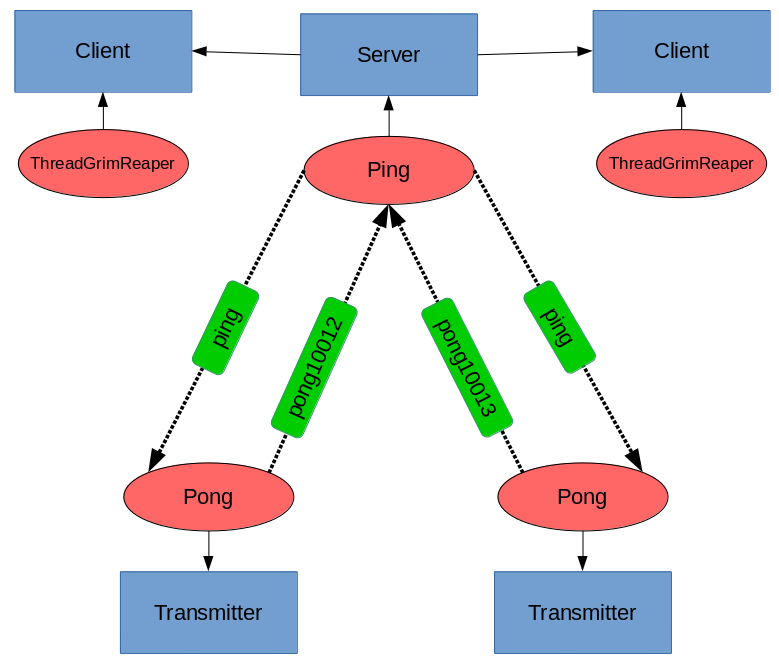
\includegraphics[scale=0.5]{Assets/s_r_3.png}
        \caption{Schéma montrant le fonctionnent des classes \textit{Ping} et \textit{Pong}}
        \label{pingpongschema}
      \end{center}
\end{figure}

\begin{figure}[th]
      \begin{center}
        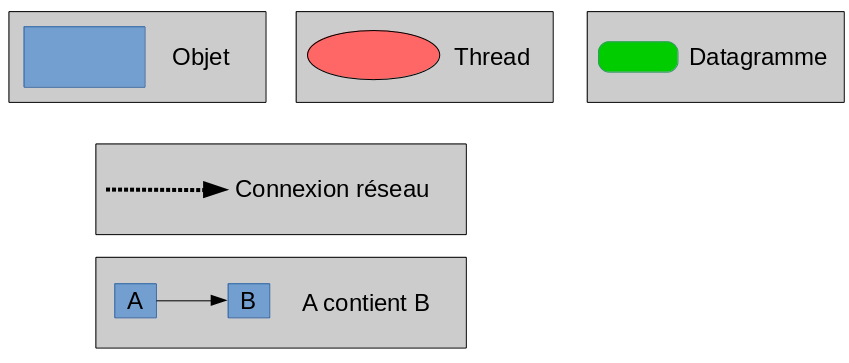
\includegraphics[scale=0.3]{Assets/l_r_3.png}
        \caption{Légende du schéma en figure \ref{pingpongschema}}
        \label{pingpongschemalegende}
      \end{center}
\end{figure}


\begin{description}
  \item[Chez le serveur : ]
  Lorsque la méthode \textit{ping\_pong()} est appelé dans la classe \textit{Server}, un thread de \textit{Ping} est créé ainsi que un thread \textit{ThreadGrimReaper}, pour chaque nouveau client. 
\textit{ThreadGrimReaper}, diminue les points de vie de 1 toutes les secondes. Si il tombe à zéro la méthode \textit{offline()} du client est appelé.
\textit{Ping} attend la réception de packages UDP sur le même port que le TCP. Lorsque un paquet est reçu \textit{Ping} récupère le code d’identification du \textit{Transmitter} dans le paquet. Puis il revoit un message «pong» à l’expéditeur, et régénéré les point de vie du client.
  
  \item[Chez le client : ]
  Lorsque la méthode \textit{ping\_pong()} est appelé dans la classe \textit{Transmitter}, un thread \textit{Pong} est créé. \textit{Pong} envoi un message UDP au serveur avec à l’intérieur son identifiant que le serveur lui a transmit lors de sa connexion. \textit{Pong} revoie en permanence un message lorsqu’il reçoit «ping». Si il ne reçoit plus de message le \textit{time out} appel la méthode \textit{offline()} du \textit{Transmitter}.
\end{description}

Grace à ces systèmes les sockets non fermé indique donc que les transmissions peuvent être effectué sans problème.


\chapter{Site web}
\section{Introduction}

	\begin{figure}[th]
		\begin{center}
		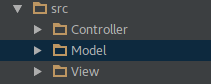
\includegraphics[scale=0.4]{Assets/mvc.png}
      		\caption{Modèle du site \textit{data wars}}
      		\label{fig1}
     		\end{center}
	\end{figure}

	Le site est construit en Modèle-Vue-Controleur. Ainsi l'ensemble des requêtes SQL se trouve dans la partie Model, les vues des pages du site sont dans la partie View et les fonctions permettant de lier la vue au modèle sont dans la partie Controller.

\section{Model}
	Dans le dossier Modele vous trouverez 3 modèles d'où vous pouvez obtenir les informations de la base de données utilisée par Data war. Ainsi vous pouvez sélectionner, ajouter, modifier et supprimer des informations :

	\begin{figure}[th]
		\begin{center}
		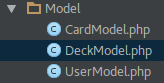
\includegraphics[scale=0.4]{Assets/modele.png}
      		\caption{Modèle du site \textit{data wars}}
      		\label{fig2}
     		\end{center}
	\end{figure}
    
	CardModel contient les requêtes SQL qui sont lié aux \textit{cartes unités et sorts} du jeu.
	DeckModel contient les requêtes SQL qui sont lié aux \textit{decks} du jeu.
	UserModel contient les requêtes SQL qui sont lié aux \textit{comptes} du site.    

\section{View}
	\begin{figure}[th]
		\begin{center}
		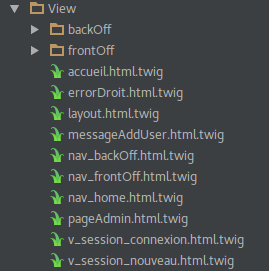
\includegraphics[scale=0.4]{Assets/view.png}
      		\caption{Vue du site \textit{data wars}}
      		\label{fig3}
     		\end{center}
	\end{figure}

	La vue se sépare en 2 sections principales :
	\begin{enumerate}
		\item le backOff
		\item le frontOff
	\end{enumerate}

	Les fichiers en dehors de ces dossiers sont les barres de navigation, la page d'accueil, les pages d'inscription au site et des pages de test.
    
	\subsection{le backOff}
        Le backOff contient les pages qui ne doivent être accessible que par les administrateurs du site, c'est à partir d'ici que la modification des cartes et des utilisateurs est possible. \textit{Il est essentiel que ces pages soient accessibles seulement aux administrateurs. }
    \begin{figure}[th]
      \begin{center}
        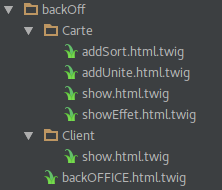
\includegraphics[scale=0.4]{Assets/backOff.png}
        \caption{Zoom sur le bloc grille}
        \label{fig4}
      \end{center}
    \end{figure}

	Comment on peut le voir ci-dessus il existe 2 dossiers :
	\begin{enumerate}
		\item Carte
		\item Client
	\end{enumerate}

	"Carte" contient les pages qui permettent de :
	\begin{enumerate}
		\item addSort : ajouter une carte sort
		\item addUnite : ajouter une carte unité
		\item showEffet : lister les effets de cartes, ajouter un effet
		\item show : lister l'ensemble des cartes présentes dans la base de donnée
	\end{enumerate}

        \subsubsection{Client}
         Dans le dossier CLient il n'y a qu'une page : "show", elle liste les comptes du site. 
        \begin{figure}[th]
      		\begin{center}
        	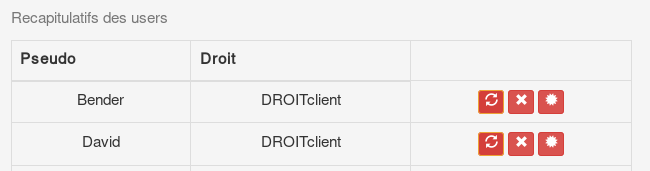
\includegraphics[scale=0.4]{Assets/liste_user.png}
        	\caption{Liste des utilisateurs}
        	\label{fig5}
      		\end{center}
    	\end{figure}

	Ainsi les selon la figure ci-dessus les options disponibles, dans l'ordre, sont : 
	\begin{enumerate}
		\item réinitialiser le deck du joueur
		\item supprimer le compte du joueur
		\item le compte obtient les droits administrateurs
	\end{enumerate}
         
	\subsection{le frontOff}
        Le frontOff contient uniquement une page qui permet au joueur de modifier son deck.
    \begin{figure}[th]
      \begin{center}
        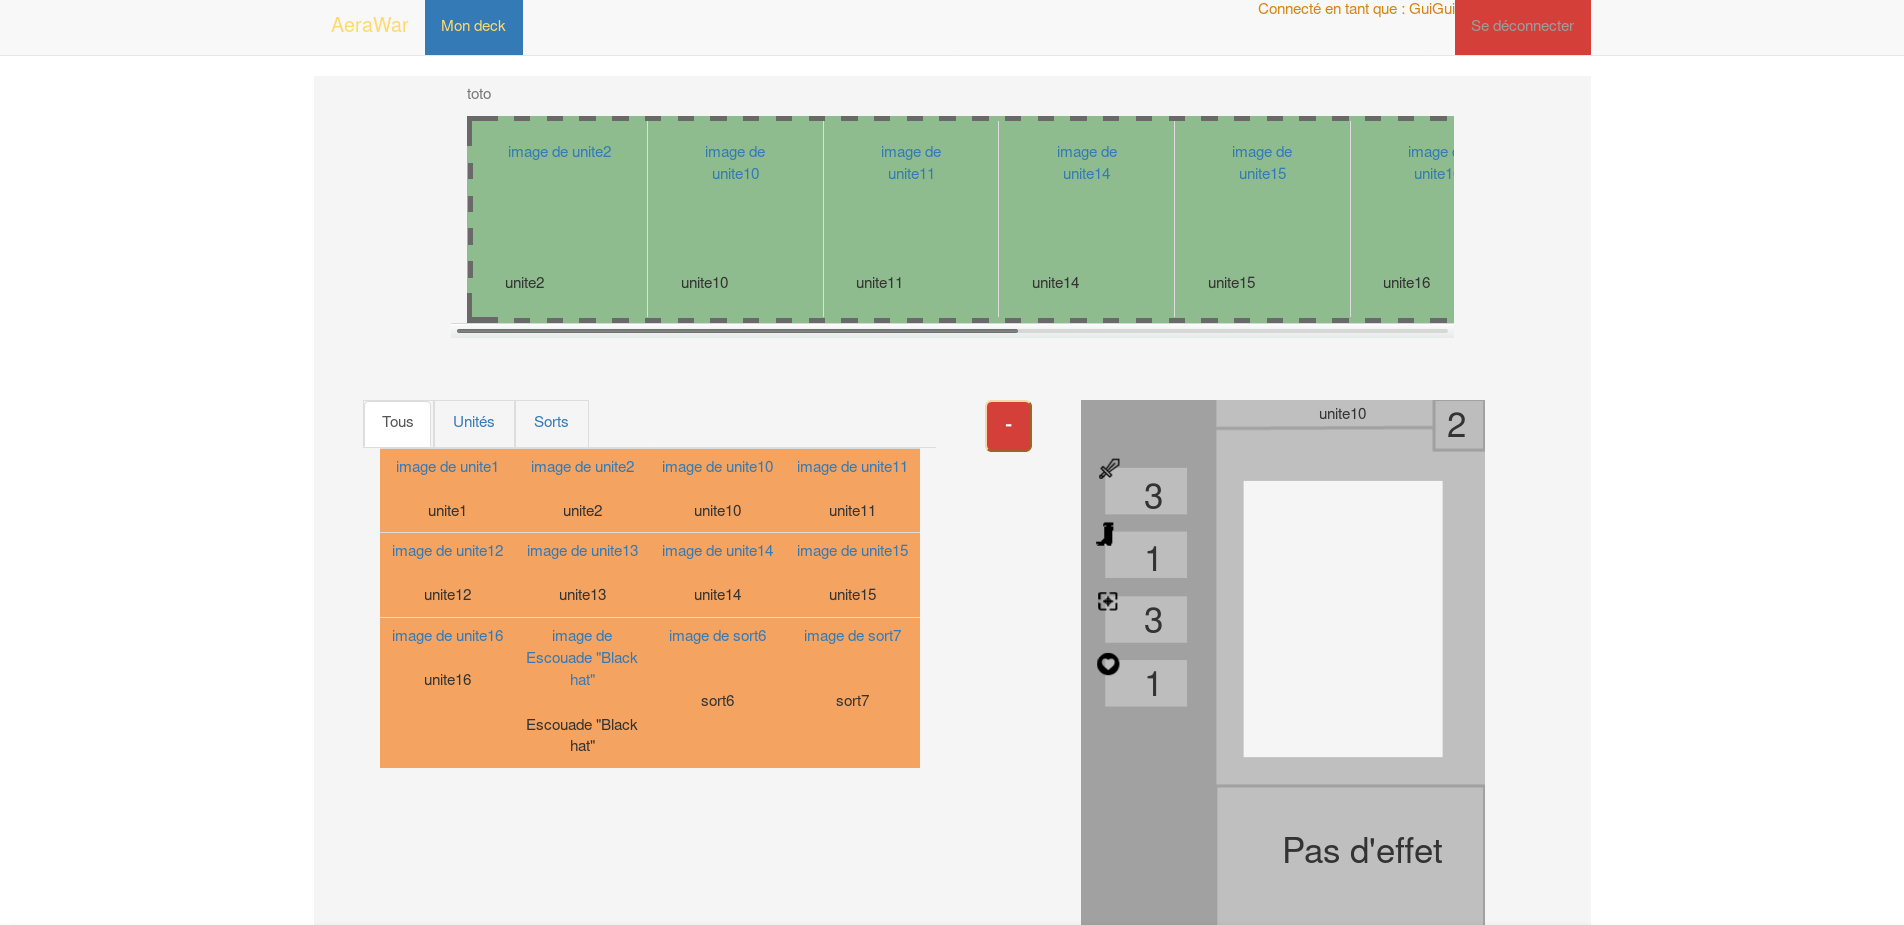
\includegraphics[scale=0.2]{Assets/site.png}
        \caption{Modfication de d'un deck}
        \label{fig6}
      \end{center}
    \end{figure}

	 La modification du deck se doit d'être confortable pour l'utilisateur. Ainsi la partie supérieure représente le deck actuel du joueur, le tableau à gauche liste l'ensemble des cartes du jeu et la carte sélectionner s'affichent sur la droite.

\section{Controller}
	Dans le dossier Controller vous trouverez l'ensemble des fonctions qui lient la vue avec le modèle.

	\begin{figure}[th]
		\begin{center}
		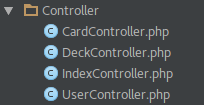
\includegraphics[scale=0.4]{Assets/controller.png}
      		\caption{Modèle du site \textit{data wars}}
      		\label{fig7}
     		\end{center}
	\end{figure}
    
	IndexController contient seulement les actions possibles pour un utilisateur non connecté à un compte. Les 3 autres fichiers sont les plus importants :

	\begin{enumerate}
		\item CardController lie les pages qui vont nécessité l'affichage des informations d'une ou plusieurs cartes
		\item DeckController permet toute les actions possible sur un deck
		\item UserController permet toute les actions possible sur un utilisateur
	\end{enumerate}

	\subsection{le contrôle des données}
	Lorsque des informations sont transmises par l'utilisateur à la base de données comme par exemple l'ajout d'une nouvelle carte il est important de procéder aux vérifications des champs de saisie. Silex nous propose de mettre en place des contraintes sur ces champs.
    \begin{figure}[th]
      \begin{center}
        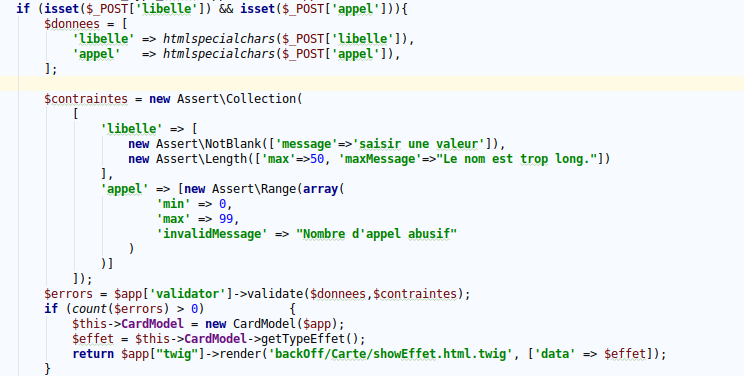
\includegraphics[scale=0.4]{Assets/exemple_contrainte.png}
        \caption{Un exemple de contrainte}
        \label{fig8}
      \end{center}
    \end{figure}

	Comment on peut le voir ci-dessus il y a 4 étapes :
	\begin{enumerate}
		\item Récupérer les données entrer
		\item Mettre en place les contraintes
		\item Comparer les données avec les contraintes
		\item Renvoyer le client à la page de saisie si une erreur est présente
	\end{enumerate}

	\subsection{Appelle des requêtes SQL}
	 \begin{figure}[th]
     		 \begin{center}
        	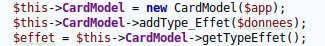
\includegraphics[scale=0.4]{Assets/requete.png}
       		 \caption{Un exemple d'utilisation de requête}
       		 \label{fig9}
     		 \end{center}
   	 \end{figure}
	
	Le code ci-dessus a pour but d'ajouter un effet dans la base de données puis de récupérer tous les effets pour enfin les envoyer sur la page "showEffet".

	Voici la procédure a suivre pour utiliser des requêtes SQL et envoyer les données sur la page de retour :
	\begin{enumerate}
		\item Initialiser une variable avec le modèle utiliser
		\item Faites l'appelle des requêtes, le retour peut être stocké dans une variable
		\item Renvoyer l'utilisateur à la page voulue, avec les données s'il y en a
	\end{enumerate}
	

      

  \listoffigures  
\end{document}  
